\documentclass{standalone}
\usepackage{tikz}
\usepackage{ctex,siunitx}
\usepackage{tkz-euclide}
\usepackage{amsmath}
\usetikzlibrary{patterns, calc}
\usetikzlibrary {decorations.pathmorphing, decorations.pathreplacing, decorations.shapes,}
\begin{document}
\small
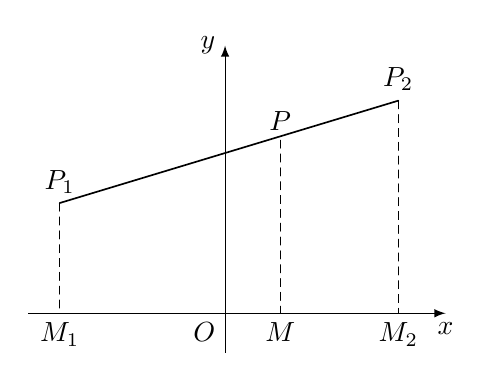
\begin{tikzpicture}[>=latex]
  \draw[thin,->](-2.5,0)--(2.8,0)node[below]{$x$};
  \draw[thin,->](0,-0.5)--(0,3.4)node[left]{$y$};
  \tkzDefPoints{0.7/2.2/P,-2.1/1.4/P1,2.2/2.7/P2,0/0/O,0.7/0/M,-2.1/0/M1,2.2/0/M2}
  % \tkzLabelPoints[below](B,C)
  \tkzLabelPoints[above](P)
  \tkzLabelPoints[below](M)
  \tkzLabelPoint[above](P1){$P_1$}
  \tkzLabelPoint[below](M1){$M_1$}
  \tkzLabelPoint[above](P2){$P_2$}
  \tkzLabelPoint[below](M2){$M_2$}
  \tkzLabelPoints[below left](O)
  \tkzDrawSegments[semithick](P1,P2)
  \tkzDrawSegments[densely dashed](P1,M1 P,M P2,M2)
\end{tikzpicture}
\end{document}